\chapter{Learning to identify clause types in English}
\label{chap:eng-cl}


As discussed in the previous chapters, cross-linguistically we see three major clause types, declaratives, interrogatives, and imperatives, dedicated to three main speech acts, assertions, questions, and commands/requests. We also see in Chapter~\ref{chap:background}, by 18 months old, infants seem to have figured out the differences among these clauses and how they are associated with their canonical functions.  To gain this ability, they must have solved a number of learning problems. Specifically, as discussed in Chapter~\ref{chap:introduction}, learners need to solve the \tbf{clustering problem}, i.e. clustering clauses in the right three categories, and the \tbf{labeling problem}, i.e. linking each category to its function. 

Given that infants's early success at identifying clause types, this chapter investigates how learners solve these problem, especially the clustering problem, by probing the extent to which children need to rely on pragmatic information (i.e., knowing what speech act a given utterance of sentence is conveying). As discussed in Chapter~\ref{chap:introduction}, pragmatic information is essential for solving the labeling problem. The question I ask here, then, is whether pragmatic information is also crucial for solving the clustering problem, as well. Will a learner strictly tracking formal regularities home in on the right three clusters of clauses? Will a learner privy to some speech act information fare better? How much pragmatic information is required? To answer these questions, I compare the performance of two computational models, a \tbf{\distlearner{}} (\dlearnerabbr{}) and a \tbf{\praglearner{}} (\plearnerabbr{}), using data from an annotated dataset I created with parental sentences in the Providence Corpus (\cite{ProvidenceCorpus}).

This rest of the chapter is organized as follows: 
In Section~\ref{sec:engcl:background}, I first briefly introduce the two computational models mentioned above, and how they can help us answer our questions (Section~\ref{sec:engcl:bg:learners}). I then review the formal features of English \diis{} (Section~\ref{sec:engcl:bg:grammar}), setting the stage for discussing the learning of these clause types. But these are features that English employs for clause typing, infants at 18 months old might not be able to perceive all (or the full-fledged version) of these features. To allow our models to best capture 18-month-olds' learning process, we need to look at 18-month-olds' linguistic capacity and knowledge with regard to these features. So in Section~\ref{sec:engcl:bg:assumptions} I briefly go through the linguistic capacities and knowledge of infants before 18 months old with regard to the formal features used for clause typing, which in turn will guide the way these features are coded in the corpus. 

In Section~\ref{sec:engcl:corpus}, I report results from a corpus study on parents' use of different clause types and speech acts, to give a quantitative description of the information present in the input. The annotated dateset result from this corpus study will be used in our modeling experiments.

Section~\ref{sec:engcl:model} details the two computational models for the two learners, \dlearnerabbr{} in Section~\ref{sec:engcl:model:baseline} and \plearnerabbr{} in Section~\ref{sec:engcl:model:pragmatics}, to see if pragmatic information is needed for solving the clustering problem. I then manipulate the ratio of noise in the pragmatic information to see how much pragmatics is needed (Section~\ref{sec:engcl:model:noisy}). Section~\ref{sec:engcl:discussion} concludes the chapter. 


\section{Background}
\label{sec:engcl:background}

\subsection{Two learners} 
\label{sec:engcl:bg:learners}
As mentioned above, the question we set out to answer is whether pragmatic information, specifically, the speech act expressed by the sentence, is necessary for learners to solve the clustering problem and find the right clause type categories. To this end, I build two computational models learning the clustering of clauses, a \text{\distlearner{}} (\dlearnerabbr{}) and a \text{\praglearner{}} (\plearnerabbr{}). Both learners are forms of distributional learning: they track distributions of certain features in their input, and use these observations to infer the underlying categories that gives rise these distributions
(cf. \cite{feldman2013,gagliardi2017modeling,perkins2022vmodel,perkins2019,nguyenwilson2021}; see \cite{pearl2020review} for a recent review). Specifically, these two learners share the same goal of discovering the underlying clustering of sentences in parents' speech, i.e. to infer the abstract clause type categories in English. The difference between them lie in the sources of information they take as input. 

The \tbf{\distlearner{}} (\dlearnerabbr{}) assumes that learners track the statistical distributions of \tit{morpho-syntactic features} present in the surface forms of sentences to infer the abstract clause type category that gives rise to these distributions. This learner serves as our baseline; by looking at its performance, we will be able to see how far syntactic information alone could take a learner in learning clause types. 

The \tbf{\praglearner{}} (\plearnerabbr{}) also tracks the distributions of morpho-syntactic features, but at the same time, it  keeps track of the speech acts expressed by these sentences as well. Thus, it infers clause type categories with information from both syntax and pragmatics. 

Thus, we would be able to answer the question of whether pragmatics is crucial for the clustering problem by comparing the performance of these two learners: if pragmatic information indeed helps the learner, not only with labeling but also with clustering, we would see \plearnerabbr{} outperforms \dlearnerabbr. Additionally, if \plearnerabbr{} indeed performs better, we can manipulate the ratio of noise in the pragmatic information that \plearnerabbr{} receives, to see how much pragmatics learners need to solve the clustering problem. 


The success of these two learners depend on the specific features we feed into the models. In Chapter~\ref{chap:background}, we have talked about speech acts extensively, but the morpho-syntactic features for clause typing differ from language to language. In the next section, we will go through the specific morpho-syntactic features that English employs for clause typing, to set the stage for our discussion of the learning of clause types. 


\subsection{Clause types in English} \label{sec:engcl:bg:grammar}

Generally, clauses in English are marked by the presence of verbs (\ref{ex:engcl:fragments}a). Sentences without verbs are often classified as fragments (\cite{sz1985speechact}), as in (\ref{ex:engcl:fragments}b):
\bex{ex:engcl:fragments}
\bxl{}
Mary hugged Ann.
\ex
Mary!
\exl
\eex

In this section, we will go over the properties of thethree major types of clauses, \diis{}, in English. 

As many have observed, the declarative clause in English tend to be ``unmarked'' (sometimes analyzed as $C$ carrying a [-int] feature) , and interrogatives and imperatives are sometimes analyzed as being the results of operations on declaratives (\cite{sz1985speechact, chomsky1957,chomsky1995minimalist, akmajian1984clausetype, platzack1997imp,rizzi1997} among many others). For example, rule $T_{q}$ in \textcite{chomsky1957} transforms a declarative sentence to an interrogative by switching the order between the subject constituent and the auxiliary constituent:
\bex{ex:engcl:chomsky:tq} 
\bxl
Structural analysis: $ \left\{\begin{array}{l}
NP-C-V \ldots\\
NP-C+M-\ldots\\ 
NP-C+\textit{have}-\ldots\\ 
NP-C+\textit{be}-\ldots 
\end{array} \right \}
$
\ex Structural change: $X_{1} - X_{2} - X_{3} \rightarrow X_{2} - X_{1} - X_{3} $
\hfill \textcite[p.112]{chomsky1957}
\exl
\eex

This rule illustrates the hallmark of interrogativity, subject-auxiliary inversion: for sentences that can be analyzed as having a subject NP followed by an auxiliary ($C$ in the structural analysis rule), apply the structural change transformation to move the auxiliary\footnote{In the case of null auxiliary (the first case), the affix rule $\#Af\rightarrow \# do+ Af$ applies to supply do-support.} in front of the subject. This trademark of [+int] value of English $C$ can be seen in polar interrogatives like  (\ref{ex:engcl:subjaux}a) and \twh-interrogatives like (\ref{ex:engcl:subjaux}b). 

\bex{ex:engcl:subjaux}
\bxl{}
Can Mary hug Ann?\hfill polar interrogative
\ex
Who can Mary hug? \hfill \twh-
interrogative
\exl
\eex


However, this association of word order and interrogativity has many exceptions. For example, in subject \twh-interrogative sentences like (\ref{ex:engcl:int-exceptions}a) and sentences with embedded interrogatives (\ref{ex:engcl:int-exceptions}b-c), the interrogative takes the same word order as a declarative. 

\bex{ex:engcl:int-exceptions}
\bxl{}
Who can hug Ann? \hfill subject \twh-interrogative
\ex
Mary wonders \tun{who Ann can hug.} \hfill embedded \twh-interrogative
\ex 
Mary wonders \tun{whether Ann can hug Sue.} \hfill embedded polar interrogative
\exl
\eex

As discussed in Chapter~\ref{chap:introduction}, these cases might be a problem for learners, as they obscure the mapping between the subject-auxiliary inversion rule and [+int]. While the presence of \twh-phrases in (\ref{ex:engcl:int-exceptions}a-b), and complementizer \tit{whether} (\ref{ex:engcl:int-exceptions}c) in these sentences are also cues for [+int], these features suffer the same problem. For example, free relative sentences (\ref{ex:engcl:whexceptions}) also appears with a clause-initial \twh-phrase, but the $C$ head this \twh-clause has the feature [-int] (\cite{bresnan1978free, caponigro2003free}):

\bex{ex:engcl:whexceptions}
Mary ate \tun{what Ann cooked.} \hfill Free relative sentences
\eex

%Mary claims that she ate what?
%in-situ \twh-questions,\footnote{We adopt the analysis given by \textcite{bobaljik2015echo} here that this type of \twh-questions are in fact declaratives with [-int] in their $C$. One of the reasons for this analysis is that these types of clauses cannot be selected by rogative verbs like \tit{wonder}:
%\begin{xlisti}
%\exi{(i)} *I wonders I should put this stuff where. \hfill (ex. (8b), \cite[p.18]{bobaljik2015echo})
%\end{xlisti}
%}


Meanwhile, some declaratives exhibit subject-auxiliary inversion as well, such as Negative Inversion sentences like (\ref{ex:engcl:neginvert}): these sentence are generally considered declaratives, but the auxiliary \tit{would} precedes the subjects in both.

\bex{ex:engcl:neginvert}
\bxl{}
Never in her life would Mary eat tripe.
\ex
Under no condition would Mary eat tripe.
\exl
\eex

These might be cases where the speech act information might be able to help, as identifying the utterance as making an assertion might help the learner avoid making the generalization that [-int] also triggers subject-auxiliary inversion. 

Imperatives (some analyzed as $C$ having the feature [imp], \cite{platzack1997imp}) in English typically use bare verb stem. In most cases, subjects are missing (\ref{ex:engcl:imp}a), but sometimes there are subjects expressing the addressee (\ref{ex:engcl:imp}b).

\bex{ex:engcl:imp}
\bxl{}
Be quiet!
\ex You be quiet!
\exl
\eex


In sum, declaratives ([-int] feature in $C$) in English are the unmarked clause type; interrogatives ([+int] in $C$) are associated with subject-auxiliary inversion, presence of clause-initial \twh-phrases, presence of complementizer \tit{whether}; imperatives ([imp] in $C$) are marked by using verb stems, and absence of sentential subjects or have second person pronouns as subjects. So to successfully infer the clause type categories, learners have to pay attention to morpho-syntactic features like the presence or absence of the sentential subject, the form of the verb, the position of the auxiliary, the presence or absence of \twh-phrases in clause-initial position, the choice of complementizers in the surface form of sentences. Table~\ref{tab:engcl:grammar} summaries the morpho-syntactic features and their associated clause types:


\begin{table}[H]
    \centering
\begin{tabular}{l|l } 
\hline
Feature  & Examples\\ 
\hline \hline
\multirow{2}{*}{$\pm$ \tsc{verb} }&
($+$) \tbf{Find} Elmo! \hfill Clause\\

&($-$) Elmo! \hfill Fragment
\\ 
\hline
\multirow{2}{*}{\tsc{$\pm$ subject} }&
($+$) \tbf{I}'ll take it. \hfill [$-$imp]\\

&($-$) Take it. \hfill [+imp]
\\
\hline
\multirow{2}{*}{\tsc{$\pm$ verb suffix} }&
($+$) Nobody feel\tbf{s} good huh? \hfill [$-$imp] \\

&($-$) Find Elmo! \hfill [+imp]
\\ 
\hline
\multirow{2}{*}{\tsc{$\pm$ subj-aux inversion} } & 
($+$) \tbf{Can you} find the ladybug? \hfill [+int]\\

&($-$) I can take it. \hfill [$-$int]
\\ 
\hline
\multirow{2}{*}{\tsc{$\pm$ sentence-initial \twh{} }} & 
($+$) \tbf{What} did you find? \hfill [+int]\\

&($-$) I found it. \hfill [$-$int] \\
\hline
\multirow{2}{*}{\tsc{complementizer} } & 
($+$) I know \tbf{whether} it's wrong. \hfill [+int]\\

&($-$) I know that it's wrong.\hfill [$-$int]
\\
\hline
\end{tabular}

\caption{Morph-syntactic features and their associated clause types}
\label{tab:engcl:grammar}

\end{table}

Of course, as we have discussed, many features do not have a one-to-one mapping with the abstract clause type categories. So apart from using the right features to cluster clauses, learners also need to avoid making certain generalizations about a feature in some cases (e.g. avoid associating subject-auxiliary inversion with declaratives upon seeing Negative Inversion sentences).  
 
While these features are significant in the grammar, it's likely that not all of these features (or the full-fledged version of these features) can be perceived by 18-month-olds. If we want to model how 18-month-olds learn clause types, the way we code these formal features in our corpus (which serves as the input to our models) has to be sensitive to their linguistic knowledge, and what they are able to perceive at the relevant age. In the next section, I will review what linguistic knowledge and capacities children have around 18th months with regard to these formal features. 

\subsection{Linguistic knowledge and capacities of 18-month-olds}
\label{sec:engcl:bg:assumptions}

Generally, infants have been shown to track distributional properties of various kinds, and 18-month-olds can perceive many grammatical features. How much do they know about the ones that associated with English \diis{} (Table~\ref{tab:engcl:grammar})? In this section, I'll briefly review 18-months-olds' capability regarding the features reviewed in the last section, and relatedly, how we code these features in our corpus. % These features are included to give the \distlearner{} the best chance of succeeding. 

\tsc{$\pm$ Verbs:} By 18 months, infants can recognize whether there is a verb in a sentence. They can use the frequent frames (e.g. adjacency to function words like auxiliaries, pronouns, or have affixes) associated with verbs to categorize a novel word as a verb (\cite{echols2004verb, mintz2006verb,peterson2006aux,soderstrom2007sv, lidzoritaomaki2012, shi2014functional, helidz2017verb} among many others), suggesting that they have knowledge of verbs, and frequent verb frames. 

\tsc{$\pm$ Verb suffixes:} Around this age, infants can recognize some morphological markings on the verb.  As early as 6 months old, English-learning infants seem to be able to segment \tit{-s, -ed, -ing} from a nonce verb (\cite{kimmegha2016morph}). 15-month-olds can segment English verbal suffix \tit{-ing} from a word, but do not do so with pseudo-suffixes (\cite{mintz2013segmentation}); 18-month-olds can distinguish well-formed auxiliary-affix dependencies (e.g. \tit{is...-ing}) vs. an ill-formed ones (e.g. \tit{can...-ing}, \cite{santelmann1998morph}). Thus, we can assume that 18-month-olds can tell whether verb suffixes are present in a sentence.

\tsc{$\pm$ Subject:} Studies have shown that infants have some knowledge about subjecthood by 18 months old.They show sensitivity to subject-verb agreement in English, as they prefer grammatical sentences over ungrammatical sentences with agreement violation (\cite{soderstrom2002agr, soderstrom2007sv, nazzi2011} among others), even if the subject is not immediately adjacent to the verb. They could also use the frame [subject pronoun + verb] to categorize novel words as verbs (\cite{babineau202014func,peterson2006aux, mintz2006verb,shi2014functional} among others). Moreover, and perhaps more important to our study, 12-month-olds are sensitive to the change in word order when the position of the subject and auxiliary is switched (\cite{geffenmintz2015wordorder}). While we do not have evidence that 18-month-olds can use the presence/absence of subjects to tell whether a sentence is imperative or not (\cite{orfitellihyams2012subj} demonstrate that 2.6-year-olds can do it), but we can assume that they can detect whether the subject is present or not.



\tsc{$\pm$ Subj-aux inversion:} By 18 months, infants can recognize whether there is an auxiliary in the sentence, and are sensitive to the relative word order between the auxiliary and the sentential subject. As mentioned above, well before they turn 18 months old, infants can already use preceding auxiliaries to categorize a novel word into the verb category (e.g. \cite{peterson2006aux, mintz2006verb}), suggesting that they understand the relation between auxiliaries and verbs. Additionally, as mentioned above, 12-month-olds can already detect subject-auxiliary inversion (\cite{geffenmintz2015wordorder}, cf. \cite{erreich1984,ambridge2006auxinvert}); with both word order and prosodic cues, even 7-month-olds are able to detect the difference between polar interrogatives and declaratives (\cite{geffenmintz2011}). We therefore assume that infants are able to detect whether there is an auxiliary in the sentence, and further they are able to detect whether the subject is preceding or following the auxiliary.

\tsc{$\pm$ Sentence-initial \twh{}:} \textcite{perkinslidz2021wh} shows that 18-month-olds, but not younger infants, begin to represent the sentence-initial \tit{which NP} as the head of a long-distance dependency. These results are suggestive, but we do not yet have evidence for the full range of \twh-phrases. In order to be conservative, we do not assume that infants have full-fledged knowledge of \twh{}. However, infants at this age are shown to have the ability to tease apart functional from content words based on their acoustic and phonological properties (\cite{shi1999func,shi2014functional}), and it is reasonable to assume that they could  \twh{s} as functional items (\cite{perkins2019}). Therefore, we will still treat \twh{} as unknown to 18-month-olds, but they are unknown \emph{functional} items (UFI), following \textcite{perkins2019}.\footnote{Note that \textcite{perkins2019} models what happens before 18 months, as her experiment narrows down the developmental window to 18 months old. Moreover, while her experiment only tests \tit{which}, there are some studies suggesting that 18-month-olds can understand \tit{what}, \tit{who}, and \tit{where} . Thus assuming that all \twh-items are unknown functional items might be too conservative. In the future, I plan to see if loosening this assumption (e.g. assume that some \twh-items are known) will boost the performance of the \dlearnerabbr{}.} We can also assume that 18-month-olds can keep track of the position of these UFIs in a sentence, so we can code \twh-items as sentence-initial UFIs. 

\tsc{Complementizer:} So far, we do not have evidence for infants' knowledge of complementizers at this age, but again they might be able to categorize complementizers as functional items. So these are treated as UFIs as well.\footnote{ Other functional items that we do not have evidence for 18-month-olds include quantifiers, focus particles, or certain conjuntors such as \tit{because}. I assume that these are UFIs as well. } Since infants can identify verbs, we assume that they can track that certain UFIs occur post-verbally. 


%Table~\ref{} summarises our assumptions about 18-month-olds' knowledge of the set of formal features that associated with clause typing.


%Finally, infants can perceive some features of prosody, and might be able to use some non-clause type-related features to infer speech acts. We will come back to both in Chapter~\ref{chap:eng-sp}.

In summary, apart from clause-initial \twh-phrases (which we assume will be perceived as clause-initial UFIs), 18-month-olds have the formal features relevant for clause typing in English. But how do parents use clause types and speech acts? How serious is the many-to-many mapping problem, between clause type and speech act, and between formal features and clause type? We will address these questions with a corpus study. %The annotated dataset resulted from this study will be used in our computational modeling experiments.

\section{Corpus study}
\label{sec:engcl:corpus}
To understand how infants figure out clause types and speech acts, we first need to establish what kind of information is present in the input. Specifically, we need to know the morpho-syntactic features of parents’ sentences, and in what contexts parents use different speech acts. For example, how available is word order as a cue to interrogativity in English-speaking parents’ speech? Are interrogative sentences associated with similar prosodic features? Do word order and prosodic features jointly correlate with interrogativity? Are there any correlations between the formal properties like syntactic and prosodic features of parents’ interrogative and their functional properties? In this section, I’ll report findings from the corpus study on parental input to English-speaking infants. 


\subsection{Corpus and Methods}
\label{sec:engcl:corpus:methods}
%%%%PAST TENSE
This study used data from the Providence sub-corpora (\cite{ProvidenceCorpus}) from CHILDES (\cite{CHILDES}), which contains conversations between 6 children and parents recorded between 2002-2005 in Providence, RI. We selected this particular corpus because it covers children’s interaction with parents at the critical age that we are interested in ($\leq$ 18 months old). Additionally, it contains transcripts, audio, and video data, providing us with an opportunity to not only look at the morpho-syntax of parents’ sentences, but also their prosodic information, and even parents’ behavior accompanying each utterance. Parent-child interaction data from five typically developing children in this corpus were included in this study: Alex, Lily, Naima, Violet, and William. %For each session, we used the transcript to annotate  

We sampled 500 conversational turns from each session with the annotation schema detailed in the next section. For the clause type and speech act information, each transcript was annotated by two annotators and compared for differences. In cases of disagreement, the two annotators would have a discussion, and if the difference cannot be resolved, a third person would be consulted. To annotate the speech act information, annotators were asked to look at 20 utterances before and 2 utterances after the current utterance in the conversation, as well as consulting the videos for contextual information. For the morpho-syntactic features, initial annotation was generated by a script (\textcolor{red}{url}) using the morphological tagging provided by CHILDES, and then manually corrected. 

In total, we annotated 9147 utterances. We will return to the video and audio part of the annotation process in Chapter~\ref{chap:eng-sp}.




\subsection{Annotation schema}
\label{sec:engcl:corpus:schema}
%As results from our corpus study would serve as input and gold standard for our models, . Our annotation schema is hence designed to capture the syntactic and prosodic features of interrogatives and their uses in the discourse. In this section, we will detail our annotation schema at each level. 
%will be coded by examining the utterance in isolation and thus in the absence of any information about the surrounding discourse. Functional features will be coded based on a combination of discourse information, the audio recordings, and the video recordings, as explained in greater detail in Section 3.2.3.  Two annotators will code the data independently and then compare for reliability. Disagreements will be settled by the two annotators by assessing the data together and, if necessary, consulting a third annotator. If a new feature category is identified as necessary, both coders will again annotate the data independently and compare for reliability. The full annotation schema can be accessed here.

\subsubsection{Clause Type}

All sentences were annotated with clause type information: declarative (\ref{eng-cl:annt:cl}a), interrogative (\ref{eng-cl:annt:cl}b), or imperative (\ref{eng-cl:annt:cl}c). Two other categories were included: Fragment and Ambiguous. In cases where the utterance only contains a noun or an injective without verbs like (\ref{eng-cl:annt:frag}), the utterance was annotated as a Fragment. In some cases, the sentence does not contain enough information to decide the clause type categories, and will thus be labelled as Ambiguous. For example, sentences like (\ref{eng-cl:annt:cl}d) could either be a case of pro-drop from the declarative sentence \tit{you want to get down}, or it could be a case of left-edge ellipsis from the polar interrogative \tit{do you want to get down}. Note that it is in principle possible to distinguish pro-drop from left-edge ellipsis; for example (\ref{eng-cl:annt:disamb}a) has to be a case of left-edge ellipsis from \tit{are you coming}, and (\ref{eng-cl:annt:disamb}b) is a case of pro-drop from \tit{I went to the store yesterday}. As the sentence in (\ref{eng-cl:annt:frag}) does not contain these morphological clues for us to make the distinction, it will be classified as Ambiguous.

\bex{eng-cl:annt:cl}	
Clause type
\bxl
\label{eng-cl:annt:decl}
It’s all twisted. \hfill Declarative
\ex \label{eng-cl:annt:int} What happened?	\hfill Interrogative
\ex \label{eng-cl:annt:imp} Throw it.\hfill Imperative
\ex \label{eng-cl:annt:frag}	Elmo!\hfill	Fragment
\ex \label{eng-cl:annt:amb} Wanna get down?	\hfill Ambiguous
\exl
\eex

\bex{eng-cl:annt:disamb}
\bxl{} You coming?\hfill Left edge ellipsis; interrogative
\ex went to the store yesterday. \hfill	Pro-drop; declarative
\exl
\eex

Interrogatives will be further divided into subcategories as polar, \twh, and disjunctive interrogatives:

\bex{eng-cl:annt:subI}	Sub-types of interrogatives
\bxl{}
Is that a big bird shovel? \hfill	Polar interrogative
\ex	Who is that?\hfill	\twh-interrogative
\ex	Do you want water or juice? \hfill Disjunctive interrogative
\exl
\eex

\subsubsection{Speech Act}

Three major speech acts categories are labelled: assertions, questions, requests/commands:\footnote{The distinction between requests and commands are subtle, and often involves the calculation of the social hierarchy between conversational partners. As parents hold authority over the child, even if the parent intend an utterance to be a request, it could be perceived by the child as a command. Therefore, we do not make a distinction in this study.}

\bex{eng-cl:annt:sp}
\bxl{} It’s all twisted!\hfill	Assertion
\ex Is that the postman?\hfill		Question
\ex Throw it!	\hfill		Request/command
\exl
\eex

As discussed in the last chapter, in many cases, one clause can used to perform both a primary speech act, and a secondary indirect speech act. For this study, we labelled the primary act performed by the utterance. For example, (\ref{eng-cl:annt:indirect}) performs a primary act of questioning and an indirect act of making a request. For these cases, the indirect speech act was annotated.

\bex{eng-cl:annt:indirect}
Can you put that down?
\eex 

\subsubsection{Formal features}

As reviewed in the last section, infants at 18 months old might have knowledge of certain morpho-syntactic features. In particular, infants might have knowledge of the subject of a sentence, its position in the sentence (whether in canonical pre-verbal position or inverted), verbs and various functional elements associated with verbs such as auxiliaries and some verbal morphology. Infants might not have a separate category for all the \twh-items, but they might be able to still classify them as functional elements, as they may know the distinction between functional and content elements. We therefore put \twh-items, quantifiers, connectives (except for \tit{and}), and focus particles in one category ``unknown functional item (UFI),'' and we annotated its position in a sentence: sentence initial, sentence-medial but before the verb, or after the verb. Each sentence was annotated with whether or not a specific feature is present. Table~\ref{tab:eng-cl:formal-schema} summarizes the features we annotated and their examples.  



\begin{table}[H]
    \centering
\begin{tabular}{l|l } 
\hline
Feature  & Examples\\ 
\hline \hline
\multirow{2}{*}{$\pm$ \tsc{verb} }&
($+$) \tbf{Find} Elmo! \hfill Clause\\

&($-$) Elmo! \hfill Fragment
\\ 
\hline
\multirow{2}{*}{\tsc{$\pm$ subject} }&
($+$) \tbf{I}'ll take it. \hfill [$-$imp]\\

&($-$) Take it. \hfill [+imp]
\\
\hline
\multirow{2}{*}{\tsc{$\pm$ verb suffix} }&
($+$) Nobody feel\tbf{s} good huh? \hfill [$-$imp] \\

&($-$) Find Elmo! \hfill [+imp]
\\ 
\hline
\multirow{2}{*}{\tsc{$\pm$ subj-aux inversion} } & 
($+$) \tbf{Can you} find the ladybug? \hfill [+int]\\

&($-$) I can take it. \hfill [$-$int]
\\ 
\hline
\multirow{2}{*}{\tsc{$\pm$ sentence-initial \twh{} }} & 
($+$) \tbf{What} did you find? \hfill [+int]\\

&($-$) I found it. \hfill [$-$int] \\
\hline
\multirow{2}{*}{\tsc{complementizer} } & 
($+$) I know \tbf{whether} it's wrong. \hfill [+int]\\

&($-$) I know that it's wrong.\hfill [$-$int]
\\
\hline
\end{tabular}

\caption{Morph-syntactic features and their associated clause types}
\label{tab:engcl:grammar}

\end{table}

\begin{table}[H]
    \centering
\begin{tabular}{r|l } 
\hline
Feature Name & Examples\\ 
\hline \hline
\multirow{2}{*}{Subject} & 
($+$) \tbf{I}'ll take it.\\
&($-$) Take it. \hfill
\\
\hline
\multirow{2}{*}{Verb} & 
($+$) \tbf{Find} Elmo! \\

&($-$) Elmo! 
\\ 
\hline
\multirow{2}{*}{Verb Morphology} & 
($+$) Nobody feel\tbf{s} good huh?\\

&($-$) Find Elmo! 
\\ 
\hline
\multirow{2}{*}{Auxilary} & 
($+$) \tbf{Can} you find it? \\

& ($-$) I found it! 
\\ 
\hline
\multirow{2}{*}{Subject-auxiliary inversion} & 
($+$) \tbf{Can you} find the ladybug?\\ %\hfill \tcb{Interrogative}

&($-$) I can take it. %\hfill\tcr{Declarative}
\\ 
\hline
\multirow{2}{*}{Sentence-initial UFI}& 
($+$) \tbf{What} did you find?\\ %\hfill \tcb{Interrogative}

&($-$) I can take it.\\
\hline
\multirow{2}{*}{Pre-verbal UFI}&
($+$) Raccoon \tbf{only} comes out at night.\\

&($-$) I can take it.\\
\hline
\multirow{2}{*}{Post-verbal UFI} & 
($+$) I know \tbf{what}'s wrong.\\

&($-$ I know you can do it.
\\
\hline
\end{tabular}

\caption{Formal features and their examples included in the corpus study}
\label{tab:eng-cl:formal-schema}

\end{table}





\subsection{Results}
\label{sec:engcl:corpus:results}


\subsubsection{Overview}
With the schema given above, an annotated dataset consisted of 9047 utterances was created. As we are primarily interested in the form and function of parents' sentences in this chapter, we excluded children's utterances and uninterpretable utterances from the dataset (as children's vocalization might change the pragmatics of the conversation, we will return to them in Chapter~\ref{chap:eng-sp}). Overall, 7039 utterances were analyzed.  Figure~\ref{fig:real-cldist} shows the distribution of clause types in the dataset. Declarative clauses are the most frequent clause type, followed by interrogatives and imperatives. 


\begin{figure}[H]
    \centering
    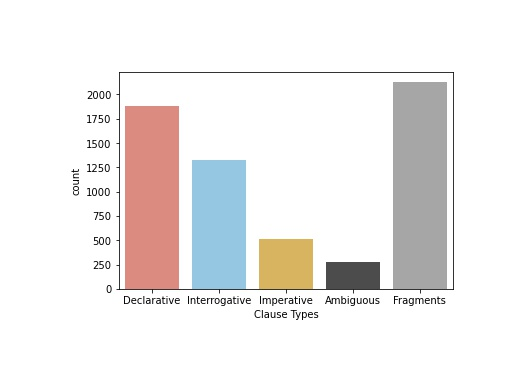
\includegraphics[width=0.7\textwidth]{figures/real-cldist.jpg}
    \caption{Distribution of clause types}
    \label{fig:real-cldist}
\end{figure}


Zooming in on interrogatives, \twh-interrogatives are more frequent than polar interrogatives; only 2 cases of disjunctive interrogatives were found in the corpus. Figure~\ref{fig:real-subI} shows the distribution of the subcategories of interrogatives. 

\begin{figure}[H]
    \centering
    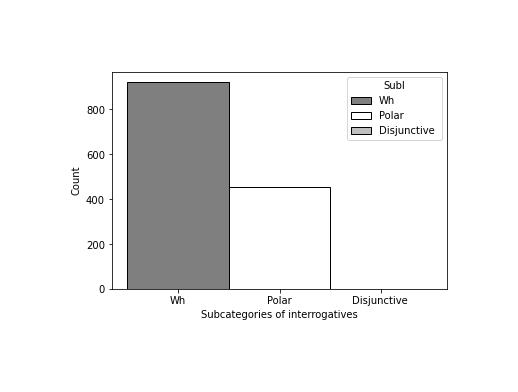
\includegraphics[width=0.7\textwidth]{figures/real-subI.jpg}
    \caption{Subcategories of interrogatives}
    \label{fig:real-subI}
\end{figure}


As shown in Figure~\ref{fig:real-clsp} and \ref{fig:real-spcl}, the mapping between speech acts and clause types are in fact quite straightforward. The majority of declaratives are used to express assertive force; the majority of interrogatives are used to express question force; and the majority of imperatives are used to express command/request force. 

\begin{figure}[H]
    \centering
    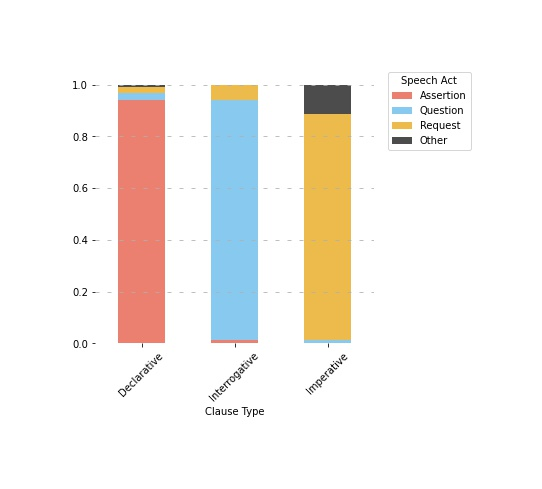
\includegraphics[width=0.7\textwidth]{figures/real-clsp.jpg}
    \caption{The speech acts performed by each clause type in parents' speech}
    \label{fig:real-clsp}
\end{figure}

Conversely, as shown in Figure~\ref{fig:real-spcl}, the majority of assertions are expressed with declaratives, questions with interrogatives, and requests with imperatives.

\begin{figure}[H]
    \centering
    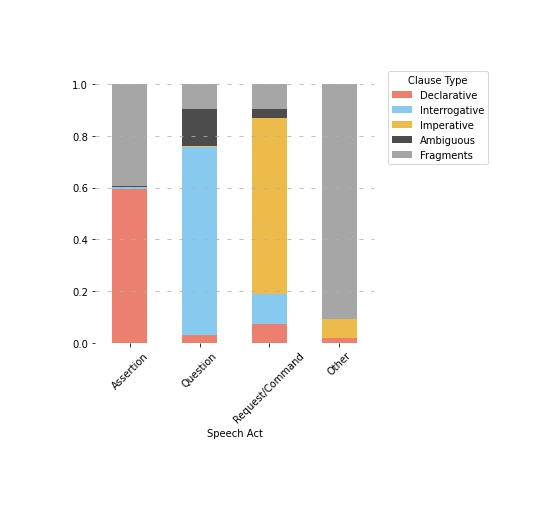
\includegraphics[width=0.7\textwidth]{figures/real-spcl.jpg}
    \caption{The clause type used to express each speech act in parents' speech}
    \label{fig:real-spcl}
\end{figure}


The few cases of mismatches seem to show systematicity as well. For example, declarative and interrogative sentences used for requests/commands tend to have modals, attitude verbs, or future morphology in the sentence:

\bex{eng-cl:dec-req}
\bxl{}	I need you to help me.		\hfill	Mother of William, Session 010605
\ex	Can you say hi?				\hfill	Mother of Lily, Session: 010117
\ex	(previous utterance: I'm gonna do some work.)\\
And you’re gonna do some coloring.\hfill		Mother of Violet, Session: 010407
\ex  Are you gonna read to Mommy?	\hfill	Mother of Lily, Session 010102
\exl
\eex 

Declarative and imperative sentences used as questions all are predominantly marked with final rise intonation. We will return to the prosodic features of each clause type in Chapter~\ref{chap:eng-sp}.

%, as in (\ref{eng-cl:dec-rise}a-b), or have embedded interrogatives (\ref{eng-cl:dec-rise}c):
\begin{comment}
\bex{eng-cl:dec-rise}
\bxl{}
Try this again?			\hfill Mother of William, Session 010605
\ex Oh , you don't wanna play with this ? \hfill	Mother of Naima, Session 001126
\ex Tell Mommy what it says. \hfill Mother of Alex, Session 010427 
\exl
\eex

\end{comment}

\begin{figure}[H]
    \centering
    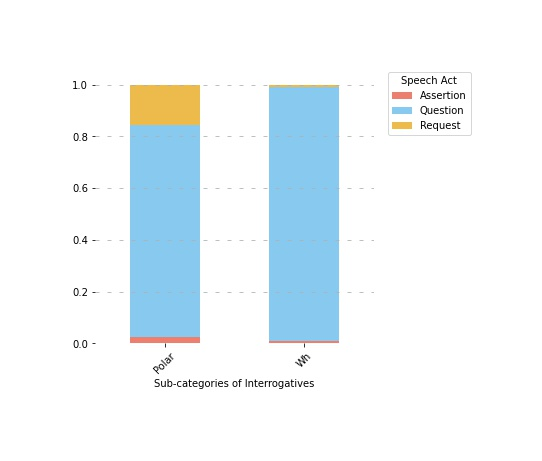
\includegraphics[width=0.7\textwidth]{figures/real-subIsp.jpg}
    \caption{The speech act expressed by different subcategories of interrogatives}
    \label{fig:real-subIsp}
\end{figure}




Turning to the speech acts of these interrogatives, Figure~\ref{fig:real-subIsp} shows the proportion of speech acts that polar and \twh-interrogatives expressed. The only two examples of disjunctive interrogatives were used both as questions, and thus not graphed in the figure. Polar interrogatives were used to express speech acts than \twh-interrogatives: around 18\% of polar interrogatives were used to indirectly raise requests like in (xx), or indirectly making an assertion like in (xx):

\bex{eng-cl:int-asst}
Polar-interrogatives as assertions:
\bxl{}
Doesn’t he have sharp teeth?	\hfill	Mother of Lily, Session: 010611
\exl
\eex

Few \twh-interrogatives were used as non-question. We found 4 cases of \twh-interrogatives used to indirectly make a request (\ref{eng-cl:wh-req}), and indirectly making assertions by way of asking rhetorical questions (\ref{eng-cl:wh-asst}):\footnote{We did also find sentences with \tit{how about/what about} (see Rawlins and Bledin 2021), but the majority of these sentences do not come with a verb and were considered fragments (\ref{eng-cl:howabout-frag}). But we also found one case of \tit{how about} interrogative with a verb (\ref{eng-cl:howabout-int}), and the primary intention of the utterance is to make a request. 

\begin{xlisti}
\ex \label{eng-cl:howabout-frag} How about this one?	\hfill	Mother of Alex Session 010512
\ex \label{eng-cl:howabout-int} How about we do these babies. \hfill	Mother of Lily, Session 010102
\end{xlisti}
}


\bex{eng-cl:wh-req}
\twh-interrogatives as requests
\bxl{}
Why don’t you turn around.	\hfill Mother of William, Session 010619
\exl
\eex
\bex{eng-cl:wh-asst}
\twh-interrogatives as assertions
\bxl{}
Who doesn’t love cheese?\hfill	Mother of Lily, Session: 010117
\ex Why are there no pens in this family?\hfill	Mother of Violet, Session: 010407
\exl
\eex




\subsubsection{Morpho-syntactic features}
\label{sec:eng-cl:corpus:formal}
We now turn to the question of how parents use each clause type, namely the formal features of each clause type. We therefore exclude fragment utterances that only contain a noun (\tit{Birdie!}), interjective (\tit{Oh}). In total, 3923 sentences were included in the analysis.

The distribution of the morpho-syntactic features listed in Table~\ref{tab:eng-cl:formal-schema} across different clause types is shown in Figure~\ref{fig:real-syncluster}. The x-axis of the figure represents the counts of sentences, and the eight morpho-syntactic features are listed along the y-axis. Each graph is split in the middle: to the left of the line, bars with darker colors represent the counts of declarative, interrogative, or imperative sentences with this specific feature, and to the right, bars with lighter colors represents the number of sentences without this feature. 





\begin{figure}[H]
    \centering
    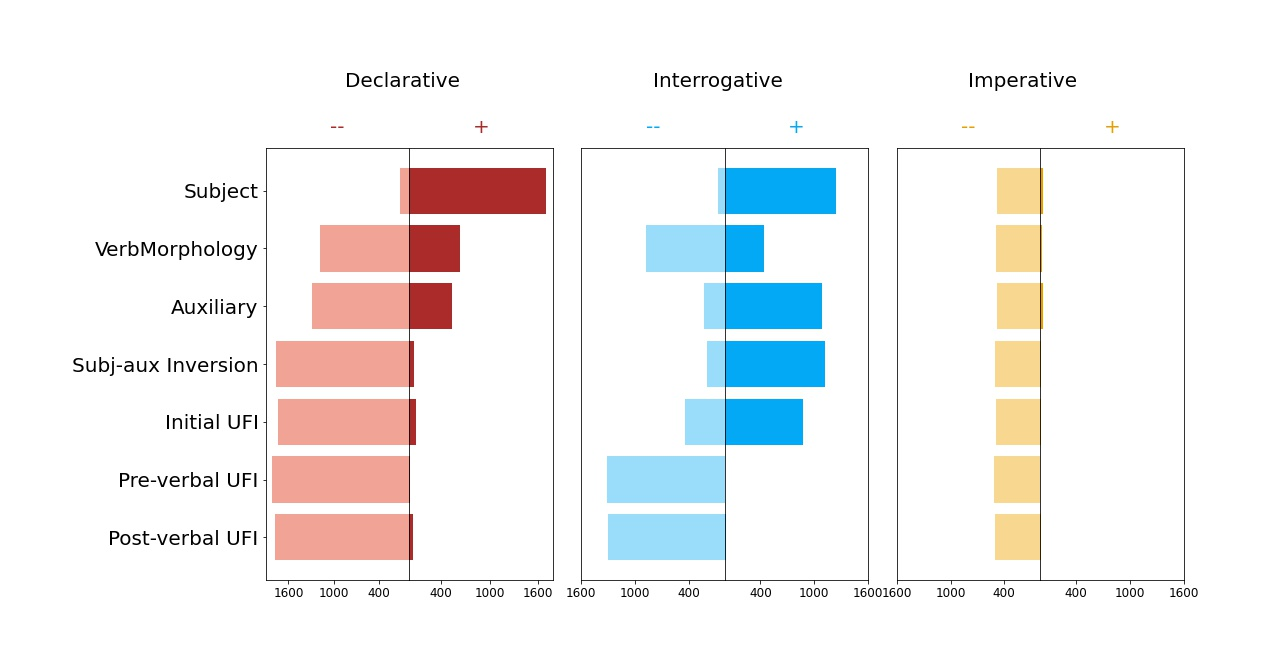
\includegraphics[width=1\textwidth]{figures/real-syncluster.jpg}
    \caption{The number of sentences with/without certain formal features in each clause type; darker color represents the number of sentences with this feature }
    \label{fig:real-syncluster}
\end{figure}

We can see that parents use the clause types rather systematically: the majority of declaratives and interrogatives are marked by the presence of subjects, as opposed to imperatives; the majority of interrogatives are marked by subjects following the auxiliary or the main verb, contrary to imperatives and declaratives; verbs in imperatives are not marked by having morphological marking on the main predicate. 

Three logistic regression models with each of the clause type as the dependent variable and the 8 morpho-syntactic features (the presence/absence of verbs and unknown functional item at preverbal position were excluded due to extremely low variance) as independent variables were performed, and the results are summarized in Table~\ref{tab:engcl:real-synstats}:


\begin{table}[H]
\begin{center}
\begin{tabular}{r|l|l|l}
\hline
 & Declaratives   & Interrogatives   & Imperatives \\
 & $\beta$  & $\beta$  & $\beta$ \\
 \hline\hline
constant & -1.7*** & -4.91*** & 1.21*** \\
\hline
Subject & 3.35*** & 1.08*** & -4.61*** \\
\hline
Verb Morphology & 1.01*** & 0.21  & -2.02*** \\
\hline
Auxiliary & 0.09  & 0.67*** & $-0.53{\cdot}$ \\
\hline
Subject-Aux Inversion & -4.2*** & 4.87*** & -1.52*** \\
\hline
Sentence-initial UFI & -2.59*** & 3.99*** & -2.38*** \\
\hline
Post-verbal UFI & -0.44  & -0.23  & $1.12{\cdot}$ \\
\hline \hline
\end{tabular}
\end{center}
\caption{Results from the three logistic regression models with each of the clause type as the dependent variable and the morpho-syntactic features as independent variables; asterisks represent the significance level: 0 ‘***’ 0.001 ‘**’ 0.01 ‘*’ 0.05 ‘$\cdot$’ 0.1 ‘ ’ 1}
\label{tab:engcl:real-synstats}
\end{table}%

From these results, we can see that the formal signatures of each clause type is consistently present in the input: auxiliary-inversion for interrogatives, the lack of auxiliary-inversion for declaratives, and lack of subject and verb morphology for imperatives. However, we do see some features that might not matter for clause typing are also present, such as the presence of subjects in declaratives and interrogatives. 

\subsubsection{Supervised learning models}
\label{sec:engcl:corpus:supervised}

The logistic regression models can be understood as supervised learning process.
Comparing two learners, one using only formal distributional features, and one also using speech act information, shows how well information from formal features predicts clause type, compared to a combination of formal and pragmatic features. Being supervised learners, these two models had access to the actual clause type labels in their training data. As shown in Figure~\ref{fig:super-compare-rand}, the supervised learner with speech act information outperforms the one with only morpho-syntactic information, but the results from the two models were fairly close.


\begin{figure}[H]
    \centering
    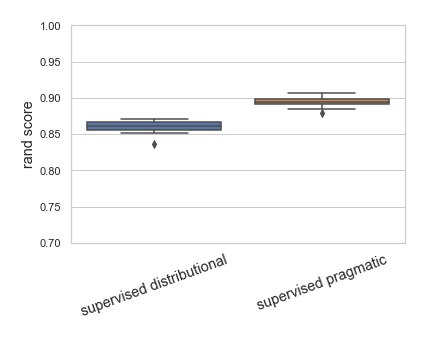
\includegraphics[width=0.6\textwidth]{figures/super-compare-rand.jpg}
    \caption{Comparing the two supervised learners by rand score (performance over 10 iterations)}
    \label{fig:super-compare-rand}
\end{figure}

Of course, these two models do not reflect \tit{how} infants learn clause typing, as they were given clause type information. A more realistic model for infant language learning would be unsupervised model where they discover the clustering of sentences. Nevertheless, the supervised learners are useful as an estimate of how informative formal and speech act features are for the task of inferring clause type.

In the next section, we will compare two \tit{unsupervised} learners that have to learn clause type categories without being trained on data annotated with the true clause type labels, which more closely mimics the learning process of language learning by infants. The \tit{distributional learner} has access to only formal features, whereas the \tit{pragmatic distributional learner} also has access to the speech act of a sentence. As we will see, in an unsupervised setting, speech act information provides a huge improvement in learners' performance.


\subsection{Interim Discussion}
\label{sec:engcl:corpus:disc}
Our corpus study provides a quantitative description of how parents use different clause types. We can see that while there are some noises, parents do use each clause type to express their canonical speech act, and each speech act is expressed by their canonical clause type. While indirect speech act exists in the dataset, their proportion is relatively low. Additionally, each clause type is systematically marked by their signature morpho-syntactic features. Interrogatives are significantly correlated with the presence of subject-initial unknown function item (e.g. \twh{}) and the auxiliary preceding the sentence subject, declaratives are correlated with the absence of these two features, and imperatives are correlated with the absence of subjects and verb morphology.  



%In the next section, we will turn to \tit{how} infants might use the information in their input to learn clause type clustering.



\section{Modeling the learning of clause types}
\label{sec:engcl:model}

In the sections below, I will report results from two learners: a distributional learner with only information about formal features (Section~\ref{sec:engcl:model:baseline}), and a pragmatic distributional learner that also takes into account the speech act information of a sentence besides the morpho-syntactic features (Section~\ref{sec:engcl:model:pragmatics}). I will show that although the distributional learner can identify clause type clusters with some success, two of the clusters do not match the actual clause type categories, as one cluster is a subset of the actual declaratives whereas another is a mix of actual declaratives and actual imperatives. The pragmatic distributional learner, on the other hand, is able to identify all three clause type categories and their formal features. The comparison between the two learners suggest that speech act information is not only helpful for the labeling of clause type clusters, but also is crucial for solving the clustering problem already. 

Besides comparing these two learners, I also simulated how much noise can the pragmatic distributional learner tolerate. In Section~\ref{sec:engcl:model:noisy}, I will show that the pragmatic distributional learner outperforms the distributional learner even with 85\% of noise in the speech act information they receive. 

With these simulations, I demonstrate that speech act information is extremely helpful to the learning of clause types, both to solve the clustering problem and the labeling problem, even if this source of information is noisy.




% \subsection{Baseline: supervised learning models}

% Before 
% \begin{figure}[H]
%     \centering
%     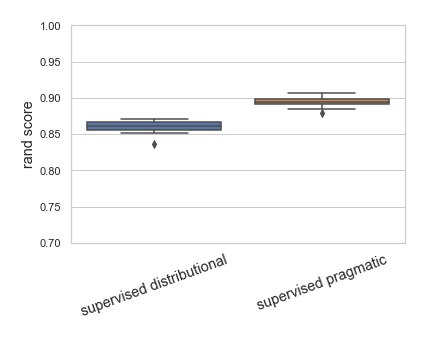
\includegraphics[width=0.8\textwidth]{figures/super-compare-rand.jpg}
%     \caption{Comparing the two supervised learners by rand score }
%     \label{fig:super-compare-rand}
% \end{figure}



\subsection{Distributional learner}
\label{sec:engcl:model:baseline}

We will start with the distributional learner that only uses morpho-syntactic features to infer the clustering of sentences. The learner was modelled with a Bayesian Clustering Model that categorises sentences based on their surface morpho-syntactic features. I will first detail the specifications of the model, and then will present simulations of the model's inference about clause type categorization. As we will see, the distributional learner can identify one category, but two of the three categories do not match the natural clause type categories.  %where it is assumed that the learner thinks the observed formal features are generated  


\subsubsection{Model Specification}
\label{sec:engcl:model:baseline:spec}


Our distributional learner assumes that the formal features observed in a given sentence are generated because the sentence belongs to one of three clause types. Figure~\ref{fig:baseline-unplate} illustrates the core idea of this model. The distributional learner assumes that a speaker generates a sentence in the following way: they first decide what clause type to use, and then decide which morpho-syntactic features need to present in the sentence given this clause type. The task of the learner is then to infer which category this sentence belongs to (i.e. the value of variable $C$, which cannot be directly observed) from the set of formal features $\vec{S}$ present/absent in the sentence (i.e. the value of Subject variable, Verb Morphology variable, subject-auxiliary inversion variable, etc., which can be directly observed and thus represented by shaded circles in the figure). The formal features included in $\vec{S}$ were the same as the set of formal features in Table~\ref{tab:eng-cl:formal-schema} in Section~\ref{sec:engcl:corpus:schema}.

\begin{figure}[H]
    \centering
    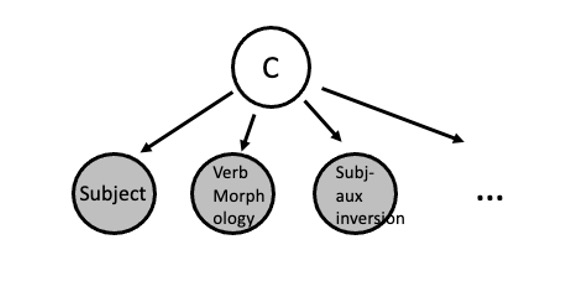
\includegraphics[width=0.5\textwidth]{figures/baseline-update.jpg}
    \caption{An illustration of the distributional learner}
    \label{fig:baseline-unplate}
\end{figure}

\begin{figure}[H]
\begin{center}
\begin{tikzpicture}
\node[latent] (c) {$C_{i}$};
\node[obs, below=of c, xshift=-0.6cm] (s) {$\vec{S_{i}}$};
\node[latent, left=of c] (phi) {$\phi^{a}$};
\node[const, left=of phi] (beta) {$\beta$};
\node[latent, left=of s] (delta) {$\delta^{c}$};
\node[const, left=of delta] (gamma) {$\gamma$};


\edge {phi}{c};
\edge {delta, c}{s};
\edge {beta}{phi};
\edge {gamma}{delta};


\plate {nutt}{(c)(s)}{$N$};
\plate {cvalue}{(delta)}{$C$};
\plate {fvalue}{(gamma)(delta)(s)(cvalue)}{$F$};
\end{tikzpicture}
\end{center}
\caption{Distributional learner}\label{fig:baseline-model}
\end{figure}

As we assume each morpho-syntactic feature follows the Bernoulli distribution, we can simplify our graph with a plate notation, with the plate $F$ representing the number of morpho-syntactic variables that the learner keeps track of (i.e. the variable $S$ repeats $F$ times). Each $S$ takes the value $1$ if the feature is present in the sentence, and $0$ otherwise. The probabilistic graphic model in Figure~\ref{fig:baseline-model} specifies the parameters and hyper-parameters of each variable with a plate notation. This learner assumes that each sentence is generated in the following way: the speaker chooses to use a certain clause type $C$, and then uses a set of morpho-syntactic features $\vec{S}$ (the number of features is $F$) to express this clause type. This process iterates $N$ times, $N$ being the number of sentences in the learner’s input. While the learner can observe the values assigned to $\vec{S}$ (represented by a shaded circle), they have to infer the value of $C$, namely their goal is to infer which clause type the speaker picked from the distribution of morpho-syntactic features of the sentence. Besides inferring the clause type of the current sentence, zooming out to the whole set of input sentences, the learner also tries to infer the probability distribution of all clause types in the input, as represented by the variable $\phi$ outside the plate $N$. Similarly, they also try to infer the probability distribution of the morpho-syntactic features ($\delta$) for each clause type across all input sentences. Namely, across all input sentences, for each clause type chosen by the speaker, how likely we would see a given feature present in the sentence. 

To put differently, the random variable $S$ is dependent on the random latent variable $C$. $C$ is in turn determined by the parameter $\phi$, which is determined by the hyperparameter $\beta$. In our model, $C$ follows multi-nominal distribution with three values, as corresponding to the three most prominent clause types (declarative, interrogative, imperative). $\vec{S}$ represents a set of morpho-syntactic features, each of which follows a Bernoulli distribution. The values for each morpho-syntactic features can be observed: if the feature is present in the current sentence, $S$ takes the value $1$, otherwise $0$. This variable is also controlled by a parameter $\delta$, indexed to $C$: each value of $C$ generates a different distribution of $\delta$ features occurring in a sentence is different depending on which clause type is being picked by the speaker. This parameter $\delta$ is controlled by a pre-determined hyper-parameter $\gamma$.


Here is a summary of the variables in the model, their meaning and distribution:

\begin{table}[H]
    \centering
    \begin{tabular}{c|l}
    \hline
    \hline
        C &  Clause Type, multinomial variable with 3 values\\
        & $ c \sim  \mbox{Multinomial}(\vec{\phi^{a}})$;\\
        &$\vec{\phi^{a}} \sim \mbox{Dir}(\beta)$\\
\hline
        $\vec{S}$ &  Morpho-syntactic features, feature bundle; \\
        & See Table~\ref{tab:eng-cl:formal-schema} for the full list of features included \\
        & $s^{(F)} \sim \mbox{Bernoulli}(\delta^{c})$ \\
        &$\delta\sim \mbox{Beta}(\gamma)$\\
    \hline
    \hline
    \end{tabular}
    \caption{Variables, their distribution, and explanation}
    \label{tab:baseline-variables}
\end{table}





\subsubsection{Inference}
\label{sec:engcl:model:baseline:infer}

The model infers the clause type category of each sentence through the method of Gibbs Sampling (\cite{geman1984gibbs}). I additionally assume the number of clause types is three. This assumption is based on the discussion that cross-linguistically, we see three major clause types: declaratives, interrogatives, and imperatives. It is therefore reasonable to start with a learner that tries to cluster the input sentences into three clusters. We will turn to the implication of this assumption, as well as propose a learner that does not adopt this assumption in Section~\ref{sec:engcl:disucssion}. 

The sampling process goes as follows. We first randomly initialize values of $C$ for each sentence with three categories (to represent declaratives, interrogatives, and imperatives). After initialization, I used the observed data in $\vec{S}$ for the current utterance and the values of $C$ of other sentences to calculate a posterior distribution over new category assignments for the current sentence, and then re-sample the new value of $C$ from this posterior probability distribution. This process was then repeated 5000 times, with the first 2500 iterations discarded as burn-in. Figure~\ref{fig:baseline-iter} shows the log of the joint probability of $C$ and $S$ at each iteration,  All parameters reached stable values within the burn-in period, and thus I will present values from the last iteration. The details of the sampling procedure and the pseudo-code of this Gibbs sampler can be found in Appendix~\ref{appx:eng-model-dir}; the code for this sampler can be found at \url{https://github.com/Yu-an/annotation_tool/blob/main/schema.pdf}. 

\begin{figure}[H]
    \centering
    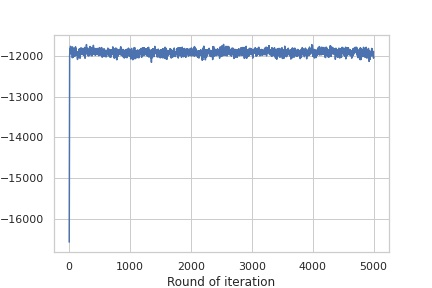
\includegraphics[width=0.7\textwidth]{figures/baseline-iter.jpg}
    \caption{The log of the joint probability $p(C,\vec{S})$ at each iteration}
    \label{fig:baseline-iter}
\end{figure}


\subsubsection{Prediction} 
\label{sec:engcl:model:baseline:predict}
This learner simulates the learning process of infants, namely that the learning of clause type clustering happens in an unsupervised setting. We therefore predict that the model would not perform as well as a supervised learner who is given the true labels of clause type. 

Additionally, this learner serves as the baseline for our pragmatic syntactic bootstrapping learner, as it only learns the clustering of sentences from morpho-syntactic features. If this learner can achieve relatively good performance, our next question is then how much information from speech act (and socio-pragmatic information) contribute to the learning of clause types.


\subsubsection{Results}
\label{sec:engcl:model:baseline:results}

The data for this model were taken from the annotated dataset reported in the last section. The relevant features included in the model are: the presence/absence of subject, verb, verb morphology, auxiliary, subject-auxiliary inversion, sentence-initial unknown functional items, non-sentence-initial but pre-verbal unknown functional items, and post-verbal unknown functional items. We further filtered out sentences without verbs, as these fragments might not contain information about clauses, and it is possible that learners could make the distinction already at this age. The true labels of clause type were used to evaluate the performance of the model. As the learner needs to learn from sentences about clause-level properties, instead of one-noun utterances or utterances of only injectives, we eliminated from the dataset sentences that do not contain a verb or an auxiliary. In total, $3923$  sentences were fed into the model.


% \begin{figure}[H]
%     \centering
%     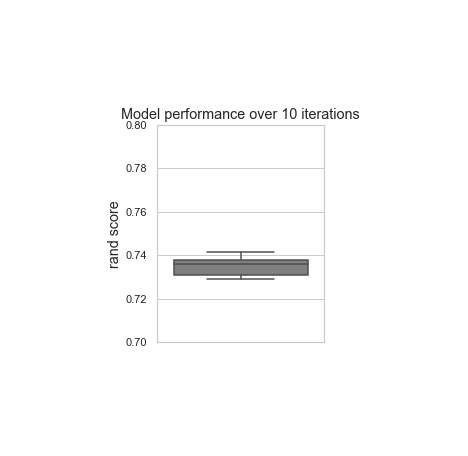
\includegraphics[width=0.5\textwidth]{figures/baseline-rand.jpg}
%     \caption{Performance of the model over 10 iterations measured by rand score}
%     \label{fig:baseline-rand}
% \end{figure}
Figure~\ref{fig:dist-compare-rand} shows the performance the distributional learner (10 rounds of simulation), in comparison to the supervised distributional learner. Rand score measures how similar the clustering result is to its gold-standard grouping; the closer the score is to 1, the better the performance. As expected, the distributional learner scores lower than the supervised learner. As will be seen, the main problem for the distributional learner comes from declaratives and imperatives, as a proportion of declaratives are clustered together with imperatives.

\begin{figure}[H]
    \centering
    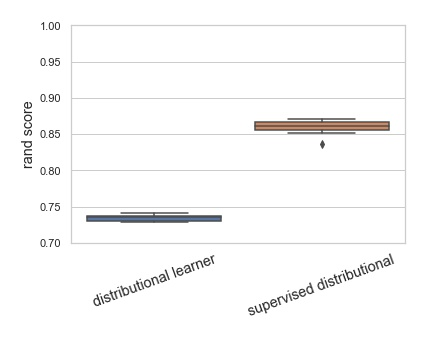
\includegraphics[width=0.6\textwidth]{figures/dist-compare-rand.jpg}
    \caption{The performance of the distributional learner and the supervised distributional learner compared by rand score }
    \label{fig:dist-compare-rand}
\end{figure}


Figure~\ref{fig:baseline-heatmap} shows how much \diis{} in each cluster identified by the model. As can be seen, Cluster~$0$ contains 90\% of interrogative clauses and Cluster~$2$ is mostly declaratives. Cluster~$1$ is split between declaratives and imperatives.

\begin{figure}[H]
    \centering
    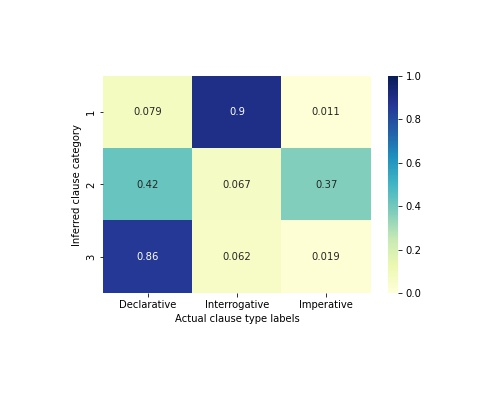
\includegraphics[width=0.7\textwidth]{figures/baseline-heatmap.jpg}
    \caption{The proportion of \diis{} in each of the three clusters}
    \label{fig:baseline-heatmap}
\end{figure}

Figure~\ref{fig:baseline-heatrev} shows the proportion of sentences clustered together. We can see that 87\% of interrogatives and 93\% of imperatives are clustered together in Cluster~$0$ and $1$ respectively. While most of declaratives are classified in Cluster~$2$, a proportion is classified in Cluster~$1$.

\begin{figure}[H]
    \centering
    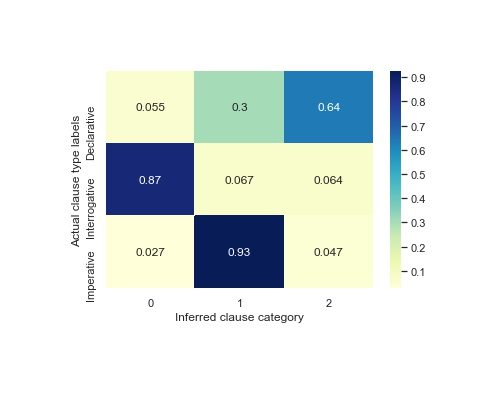
\includegraphics[width=0.7\textwidth]{figures/baseline-heatrev.jpg}
    \caption{The proportion of actual \diis{} clustered in one category}
    \label{fig:baseline-heatrev}
\end{figure}

The distribution of formal features in each cluster is shown in Figure~\ref{fig:baseline-syncluster}, and three logistic regression models with each of the clusters as dependent variable, and the set of formal features (+/- verb and pre-verbal UFI are excluded, due to low variance) as independent variable are performed. Results of which is shown in Table~\ref{tab:baseline-synstats}.

\begin{figure}[H]
    \centering
    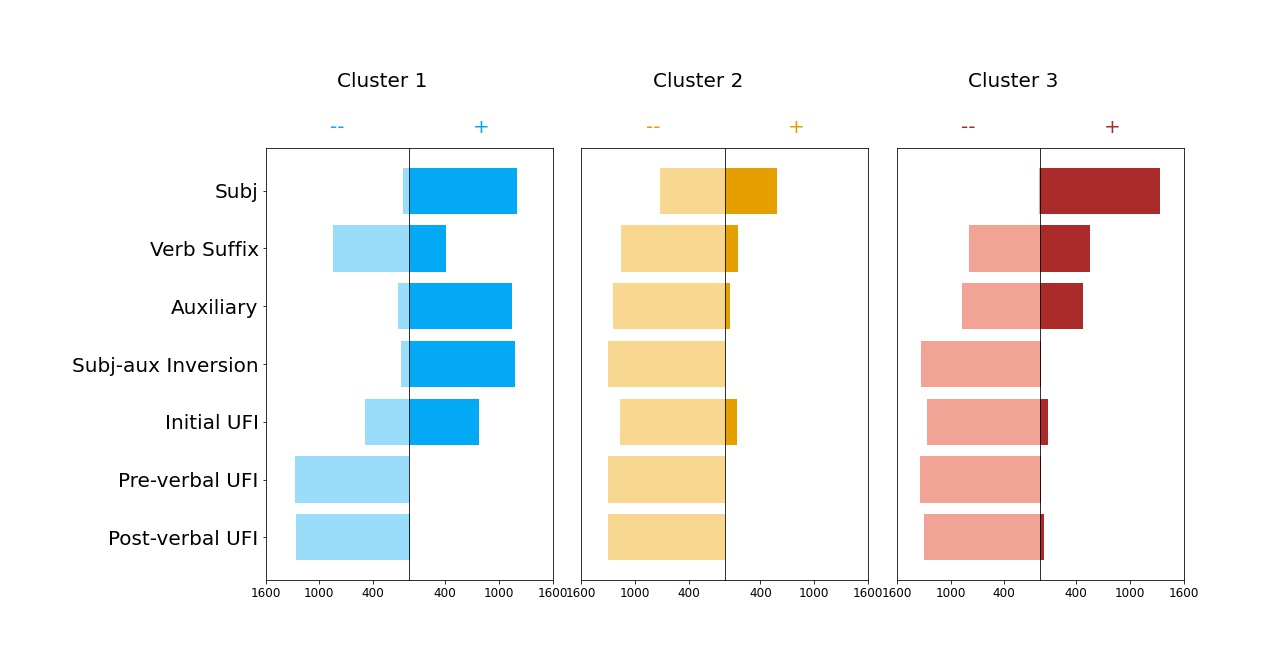
\includegraphics[width=1\textwidth]{figures/baseline-syncluster.jpg}
    \caption{The number of sentences with/without certain formal features in each cluster (Cluster 0 $\sim$ Interrogatives, Cluster 1 $\sim$ Imperatives, Cluster 2 $\sim$ Declaratives), darker colors represent the number of sentences with the feature. UFI stands for Unknown Functional Item (e.g. \twh{}), see Table~\ref{tab:eng-cl:formal-schema} for details.}
    \label{fig:baseline-syncluster}
\end{figure}

\begin{table}[H]
\begin{center}
\begin{tabular}{r|l|l|l}
\hline
 & Cluster~$0$   & Cluster~$1$   &  Cluster~$2$ \\
 & $\sim$ Interrogatives  & $\sim$ Imperatives  & $\sim$ Declaratives \\
 \hline\hline
constant & -6.97*** & 4.461*** & -4.22*** \\
\hline
Subject & 1.00* & -4.49*** & 4.37*** \\
\hline
Verb Morphology & -1.56*** & 0.21  & -1.46*** \\
\hline
Auxiliary & 3.4***  & -2.72*** & 1.16*** \\
\hline
Subject-Aux Inversion & 7.45*** & -5.83*** & -1.52*** \\
\hline
Sentence-initial UFI & 3.08*** & 0.38* & -1.58*** \\
\hline
Post-verbal UFI & -0.51  & -3.07***  & 1.69*** \\
\hline \hline
\end{tabular}
\end{center}
\caption{Results from the three logistic regression models with each of the clusters as the dependent variable and the morpho-syntactic features as independent variables; asterisks represent the significance level: ‘***’ 0.001 ‘**’ 0.01 ‘*’ 0.05 ‘.’ 0.1 ‘ ’ 1}
\label{tab:baseline-synstats}
\end{table}%


From the above table and figure, we can see that the model clearly identifies a cluster for interrogatives, and that features associated with polar and \twh-interrogatives are both present in this cluster. Interestingly, both subject and object \twh-interrogatives are included in this cluster:
\bex{engcl:baseline:cluster0}
Who's hiding in the barrel? \hfill Mother of Violet, Session 010603
\ex What else do we have here? \hfill Mother of Naima, Session 001126
\eex

Thee other two clusters are not as ideal. Cluster~$1$ consists of a mix of imperative sentences and simple declarative sentences like (\ref{engcl:baseline:cluster1-dec}):

\bex{engcl:baseline:cluster1-dec}
It's moon face. \hfill Mother of Lily, Session 010423
\ex I love school. \hfill Mother of Lily, Session 010423
\eex

Ambiguous sentences (sentences that could either be a pro-drop declarative or an left-edge-ellipsis interrogative) like \ref{engcl:baseline:cluster1-amb} are also put in Cluster~$1$:
\bex{engcl:baseline:cluster1-amb}
Wanna read your little Tigger book? \hfill Mother of Violet, Session 010407
\eex


Overall, the distributional learner fails to identify two of the three clause types in English, and fails to identify the characteristic features for imperatives and declaratives. We will turn to the pragmatic distributional learner next, to evaluate whether the learner needs information from pragmatics to identify clause types.

%As we have discussed, infants do not have access to the real labels of clause types. A more realistic model for infant language learning would be unsupervised model where they discover the clustering of sentences. In the next sections, we will compare two learners that have to learn clause type categories without access to the true labels, which mimics the learning process of language learning by infants: the distributional learner and the pragmatic distributional learner. 


\subsection{Pragmatic distributional learner}
\label{sec:engcl:model:pragmatics}

As we have discussed in Section~\ref{sec:engcl:background}, the learner needs to solve two problems: clustering the sentences, and labeling the clusters. We additionally see that speech act information is necessary to solving the labeling problem. The question then is, do learners need this information source to solve the clustering problem. As clause type categories are formal categories, theoretically we might not need information from the function of a sentence to identify these formal categories. However, as we have seen in the last section, a learner with only formal features cannot identify all three clause types. In this section, we will test the pragmatic distributional learner, to see if their performance improves.

Using speech act information also does not necessarily means that the performance of the learner improves, since speech acts could potentially be expressed by any type of clause type, and vice versa. It remains to be seen whether this source of information helps the learner or hurts the learner. 

We have seen in Section~\ref{sec:engcl:corpus:supervised}, in a supervised learning setting where the model is trained on actual clause type category data, adding pragmatics to the model improves model performance. But we also discussed that infants are not given the actual labels. In this section, we are building the pragmatic distributional learner with a Bayesian Clustering Model again, where the model infers clause type clustering without actual clause type labels. 

In this section, I will first detail the specification of the pragmatic distributional learner, which is given speech act information and information about morpho-syntactic features, to infer clause typing. I then compare the performance of the two learners (and their supervised counter-parts). As we will see, the pragmatic distributional learner outperforms the distributional learner. Speech act also provides a much higher performance boost for our unsupervised learners, as the improvement is much higher than their supervised counterparts.


\subsubsection{Model Specification}
\label{sec:engcl:model:prag:spec}


Similar to the distributional learner, the pragmatic distributional learner is also a Bayesian Clustering Model. The learner is given speech act information ($A$) in addition to the morpho-syntactic features ($\vec{S}$). The pragmatic distributional learner assumes that each sentence is generated in the following way: the speaker of the sentence first chooses a particular speech act ($A$), then picks one out of three clause types to express the speech act, and finally picks what kind of formal figures to use. 



\begin{figure}[H]
\begin{center}
\begin{tikzpicture}
\node[obs] (a) {$A_{i}$};
\node[latent, left=of a] (theta) {$\theta$};
\node[const, left=of theta] (alpha) {$\alpha$};
\node[latent, below=of a] (c) {$C_{i}$};
\node[obs, below=of c, xshift=-0.6cm] (s) {$\vec{S_{i}}$};
\node[latent, left=of c] (phi) {$\phi^{a}$};
\node[const, left=of phi] (beta) {$\beta$};
\node[latent, left=of s] (delta) {$\delta^{c}$};
\node[const, left=of delta] (gamma) {$\gamma$};

\edge {theta}{a};
\edge {alpha}{theta};
\edge {phi, a}{c};
\edge {delta, c}{s};
\edge {beta}{phi};
\edge {gamma}{delta};


\plate {nutt}{(a)(c)(s)}{$N$};
\plate {avalue}{(phi)}{$A$};
\plate {cvalue}{(delta)}{$C$};
\plate {fvalue}{(gamma)(delta)(s)(cvalue)}{$F$};
\end{tikzpicture}
\end{center}
\caption{Pragmatic distributional learner}\label{fig:target-model}
\end{figure}

Figure~\ref{fig:target-model} shows the graphical model of the learner. The model assumes that the latent variable $C$ depends on the value of an observed variable $A$. This variable $A$ follows a multi-nominal distribution with parameter $\theta$, representing the probability distribution of each speech act in the input. The parameter for $C$ is still $\phi$, but this time $\phi$ is indexed to values of $A$, namely for each speech act, the distribution over different clause types might be different. Similar to the distributional learner, morpho-syntactic features are again represented by $\vec{S}$, which contains a set of formal features (the same ones as in the distributional learner). $\vec{S}$ is dependent on $C$ and the parameter $\delta$. 

This learner's task is to infer the category $C$ of each sentence with the observed surface formal features, as well as the speech act information. In this section, we assume that the learner has access to the speech act information. Here our goal is to simply test the idea that if the learner is given data about the function of a clause, will its performance in solving the clustering problem improve.

In the next section, we will examine how much information from speech act the learner actually needs by manipulating the amount of noise in speech act information. One might wonder how children might bootstrap into the different speech act categories in the first place. We will turn to some possible sources for speech act categorization in Chapter~\ref{chap:eng-sp}.

Besides trying to infer the value of $C$ for each utterance, the learner also needs to learn the probability distribution of each clause type associated with each speech act. Note that this is a rather simplified representation of the relation between clause type and speech act, further research is needed to model the relationship between form and function (see \cite{gong2021rsaq} for an attempt to use rational speech act theory to capture this form-function relation).



Here is a summary of the variables in the model, their meaning and distribution:

\begin{table}[H]
    \centering
    \begin{tabular}{c|l}
    \hline
    \hline
    
        A & Speech Act, four values: Assertion, Question, Request/Command, other\\
        & $ a \sim \mbox{Multinomial}(\vec{\theta})$;\\
        & $\vec{\theta} \sim \mbox{Dir}(\alpha)$\\
\hline
        C &  Clause Type, multinomial variable with 3 values\\
        & $ c \sim  \mbox{Multinomial}(\vec{\phi^{a}})$;\\
        &$\vec{\phi^{a}} \sim \mbox{Dir}(\beta)$\\
\hline
        $\vec{S}$ &  Syntactic features, feature bundle; \\
        & the value of each feature $F$ is $S^{(F)}$ \\
        & $s^{(F)} \sim \mbox{Bernoulli}(\delta^{c})$ \\
        &$\delta\sim \mbox{Beta}(\gamma)$\\
    \hline
    \hline
    \end{tabular}
    \caption{Variables in the pragmatic distributional learner, their distributions, and explanations}
    \label{tab:target-variables}
\end{table}


\subsubsection{Inference}
\label{sec:engcl:model:prag:infer}




The sampling process is similar to that in the last section. We first randomly initialize values of $C$ for each sentence with three categories (to represent declaratives, interrogatives, and imperatives). After initialization, I use the observed data in $A$ and the observed data in $\vec{S}$ for the current utterance and the values of $C$ of other sentences to calculate a posterior distribution over new category assignments for the current sentence, and then re-sample the new value of $C$ from this posterior probability distribution. Again, a Gibbs sampler similar to that for the baseline model was implemented, and the sampling procedure repeated for 5000 times with the first 2500 discarded as burn-in. Values of all parameters converged to a stable state within the burn-in period, and therefore the values from the last iteration will be reported here.  Figure~\ref{fig:baseline-iter} shows the log of the joint probability of $C$ and $S$ at each iteration.  All parameters reached stable values within the burn-in period, and thus I will present values from the last iteration. %The details of the sampling procedure and the pseudo-code of this Gibbs sampler can be found in Appendix~\ref{appx:eng-model-dir}; the code for this sampler can be found URL. 

\begin{figure}[H]
    \centering
    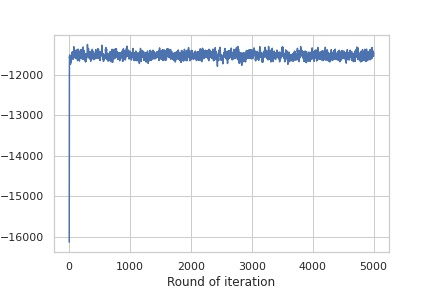
\includegraphics[width=0.7\textwidth]{figures/target-iters.jpg}
    \caption{The log of the joint probability p(A,C,$\vec{S}$) across 5000 iterations}
    \label{fig:target-iters}
\end{figure}




\subsubsection{Prediction}
\label{sec:engcl:model:prag:predict}


If learners do need function information to cluster sentences, we will see the pragmatic distributional learner outperforms the distributional learner. However, this learner is still an unsupervised learner, in that it is not trained on the actual clause type labels in the corpus, so its performance might be lower than the supervised models.



\subsubsection{Results}
\label{sec:engcl:model:prag:results}

We draw the data for simulation from the same dataset, this time with speech act information. Overall, the model outperforms the distributional learner. As can be seen from Figure~\ref{fig:compare-rand}, the rand score (which measures how well two clusters coincide with each other) of the pragmatic distributional learner is higher. Additionally, the difference between the pragmatic and the distributional learner is larger than the difference between the two supervised learners, suggesting that for learners without access to the actual labels of clause types (which we assume to be the best approximation to the language acquisition process of infants), speech act information is crucial not only for labeling, but also clustering. 


\begin{figure}[H]
    \centering
    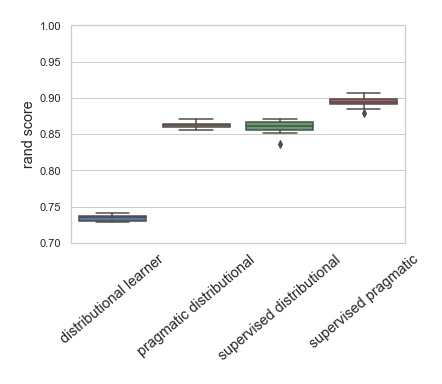
\includegraphics[width=0.6\textwidth]{figures/compare-rand.jpg}
    \caption{Comparing all four learners (distributional, pragmatic distributional, supervised distributional, supervised pragmatic) by rand score }
    \label{fig:compare-rand}
\end{figure}




Figure~\ref{fig:target-heatmap} shows how much \diis{} in each cluster identified by the model. As can be seen, the model is able to identify three clause clusters: Cluster~$0$ contains 94\% of interrogative clauses, Cluster~$2$ is mostly imperatives, and Cluster $1$ mostly declaratives. 

\begin{figure}[H]
    \centering
    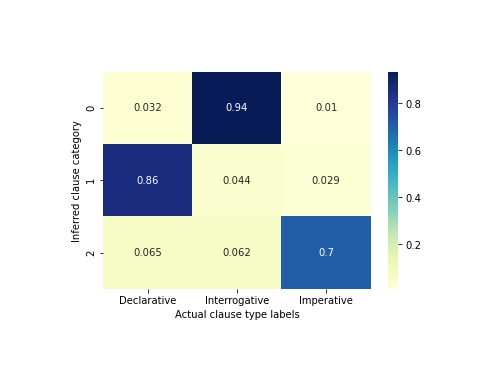
\includegraphics[width=0.7\textwidth]{figures/target-heatmap.jpg}
    \caption{The proportion of \diis{} in each of the three clusters}
    \label{fig:target-heatmap}
\end{figure}

Figure~\ref{fig:target-heatrev} shows the proportion of sentences clustered together. We can see that our learner performs extremely well: 95\% of declaratives, 90\% of interrogatives, and 87\% of imperatives are clustered together in Cluster~$1$, $0$, $2$ respectively.


\begin{figure}[H]
    \centering
    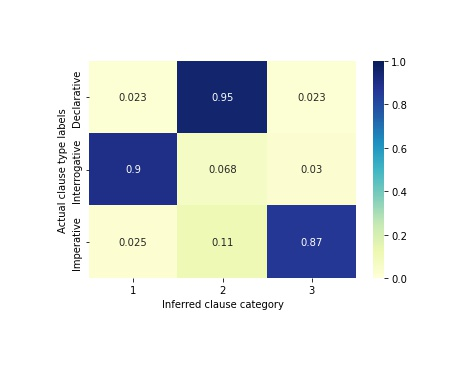
\includegraphics[width=0.7\textwidth]{figures/target-heatrev.jpg}
    \caption{The proportion of actual \diis{} clustered in one category}
    \label{fig:target-heatrev}
\end{figure}


Figure~\ref{fig:target-syncluster} shows the presence of morpho-syntactic features in each cluster; Table~\ref{tab:target-synstats} summarises the three logistic regression models with each of the clusters as dependent variable, and the set of formal features (+/- verb and pre-verbal UFI are excluded, due to low variance) as independent variables.  

\begin{figure}[H]
    \centering
    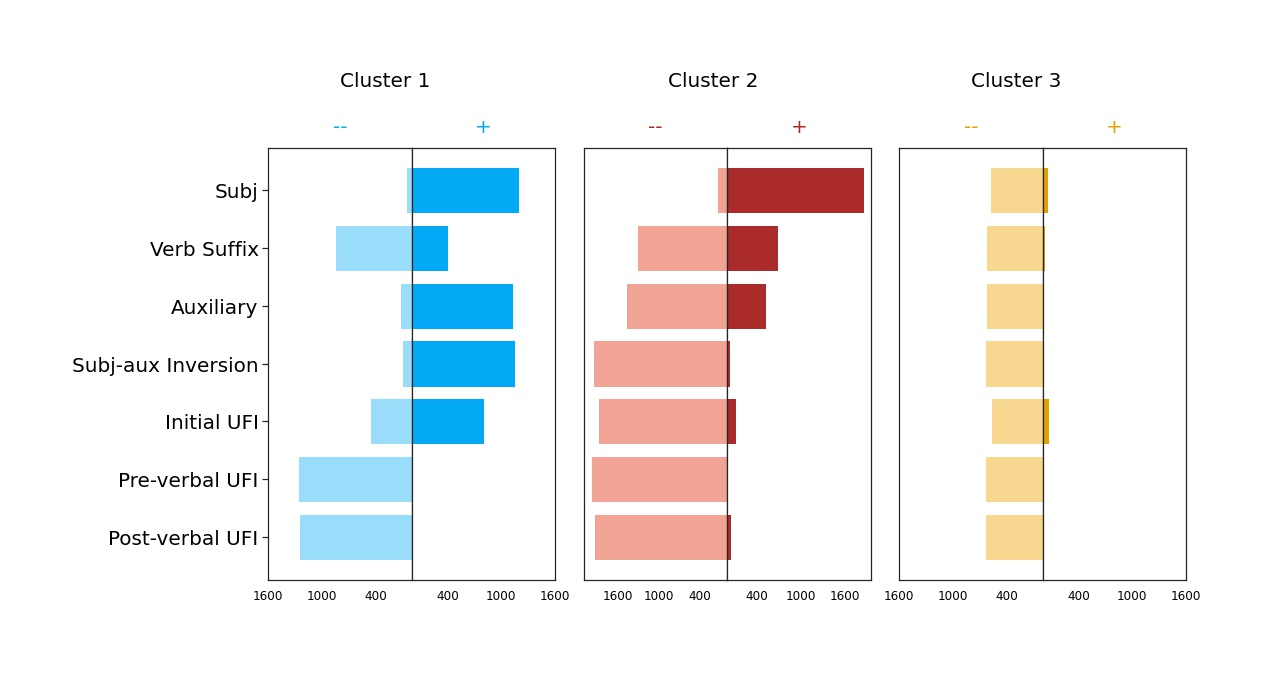
\includegraphics[width=1\textwidth]{figures/target-syncluster.jpg}
    \caption{The number of sentences with/without certain formal features in each cluster (Cluster 0 $\sim$ Interrogatives, Cluster 1 $\sim$ Declaratives, Cluster 2 $\sim$ Imperatives), darker colors represent the number of sentences with the feature.}
    \label{fig:target-syncluster}
\end{figure}


\begin{table}[H]
\begin{center}
\begin{tabular}{r|l|l|l}
\hline
 & Cluster~$0$   & Cluster~$1$   &  Cluster~$2$ \\
 & $\sim$ Interrogatives  & $\sim$Declaratives  & $\sim$ Imperatives \\
 \hline\hline
constant & -6.3*** & -1.44*** & 1.95*** \\
\hline
Subject & 0.9** & 4.32*** & -4.75*** \\
\hline
Verb Morphology & -0.31 & 1.66***  & -3.08*** \\
\hline
Auxiliary & 2.66***  & -0.85*** & -2.14*** \\
\hline
Subject-Aux Inversion &5.99*** & -5.83*** & -56.79 \\
\hline
Sentence-initial UFI & 3.65*** & 0.38* & 0.72** \\
\hline
Post-verbal UFI & -0.43  & 0.5  & -1.12 \\
\hline \hline
\end{tabular}
\end{center}
\caption{Results from the three logistic regression models with each of the clusters as the dependent variable and the morpho-syntactic features as independent variables; asterisks represent the significance level: ‘***’ 0.001 ‘**’ 0.01 ‘*’ 0.05 ‘.’ 0.1 ‘ ’ 1}
\label{tab:target-synstats}
\end{table}%

% \begin{figure}[H]
%     \centering
%     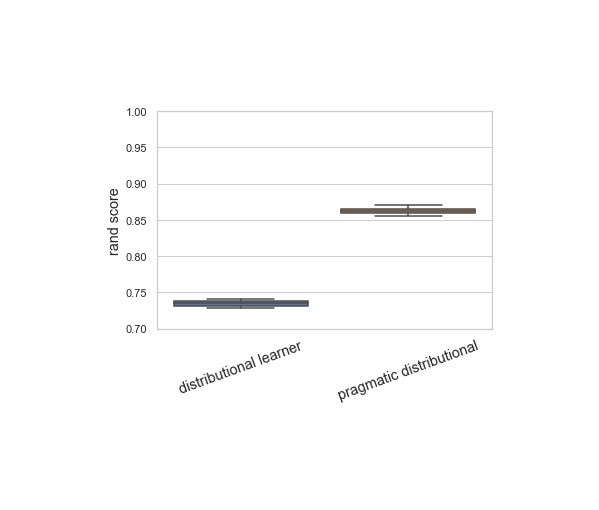
\includegraphics[width=0.6\textwidth]{figures/target-base-rand.jpg}
%     \caption{Comparing the pragmatic distributional learner and the distributional learner by rand score }
%     \label{fig:target-base-rand}
% \end{figure}


The distribution of formal features across the three clusters is similar to the distribution with actual clause type categories. Cluster $0$, the interrogative cluster, is associated with the presence of subject-auxiliary inversion and sentence-initial unknown functional items (UFIs); Cluster $2$, the imperative cluster, is associated with the absence of subject, auxiliaries, verb morphology, or UFIs. The declarative cluster Cluster $1$ is correlated with the presence of subjects, verb morphology, and the lack of subject-auxiliary inversion. The three clusters match the actual clause types, \diis.

Comparing the pragmatic distributional learner with the distributional learner, we can see that the former performs much better, identifying all three clause types and the prominent features associated with these clusters. These results suggest the learner needs information from pragmatics to succeed in clause typing. But how much does the learner need pragmatics? Will noisy speech act information still able to help the learner? In the next section, we compare pragmatic distributional learners with different levels of noises in their speech act information, and see how well the learner performs with deprecated data.

\subsection{Noisy pragmatic distributional learner}
\label{sec:engcl:model:noisy}

\subsubsection{Simulating noisy A}
The model is the same as the pragmatic distributional learner discussed in the last section, but instead of taking true speech act labels as input, the model was fed noisy speech act information. With this manipulation, we would be able to see how much the model can handle noise from speech act information. 




\begin{figure}[H]
\begin{center}
\begin{tikzpicture}
\node[obs] (a) {$A'_{i}$};
\node[latent, left=of a] (theta) {$\theta$};
\node[const, left=of theta] (alpha) {$\alpha$};
\node[latent, below=of a] (c) {$C_{i}$};
\node[obs, below=of c, xshift=-0.6cm] (s) {$\vec{S_{i}}$};
\node[latent, left=of c] (phi) {$\phi^{a}$};
\node[const, left=of phi] (beta) {$\beta$};
\node[latent, left=of s] (delta) {$\delta^{c}$};
\node[const, left=of delta] (gamma) {$\gamma$};

\edge {theta}{a};
\edge {alpha}{theta};
\edge {phi, a}{c};
\edge {delta, c}{s};
\edge {beta}{phi};
\edge {gamma}{delta};


\plate {nutt}{(a)(c)(s)}{$N$};
\plate {avalue}{(phi)}{$A$};
\plate {cvalue}{(delta)}{$C$};
\plate {fvalue}{(gamma)(delta)(s)(cvalue)}{$F$};
\end{tikzpicture}
\end{center}
\caption{Pragmatic distributional learner}\label{fig: noisy-model}
\end{figure}

In this model, we replace the true labels of the speech act variable $A'$ with a noisy version of $A$. A portion of the observations of $A'$ will be replaced by noise. To make the simulation, I replace 0 to 100\% of the true labels of speech act information with random labels. The goal of the model is to see at what noise level would the speech act information affects the inference of clause type categories. 

I again adopt the Gibbs sampling method to infer the parameter values, same as for the last two models. The sampling procedure repeat 5000 times with the first 2500 discarded as burn-in. Values of all parameters converge to a stable state within the burn-in period, and therefore the values from the last iteration will be reported here. 

\subsubsection{Results}
\label{sec:engcl:model:noisy:results}

Figure~\ref{fig:noisy-rand-compare} shows the performance of the pragmatic distributional learner when the speech act contains 0-100\% noise. As can be seen, the learner outperforms the distributional learner up until there is around 85\% of noise in speech act. This suggests that speech act information is helpful for learners to cluster sentences, and even deprecated speech act information will still help the learner.  

\begin{figure}[H]
    \centering
    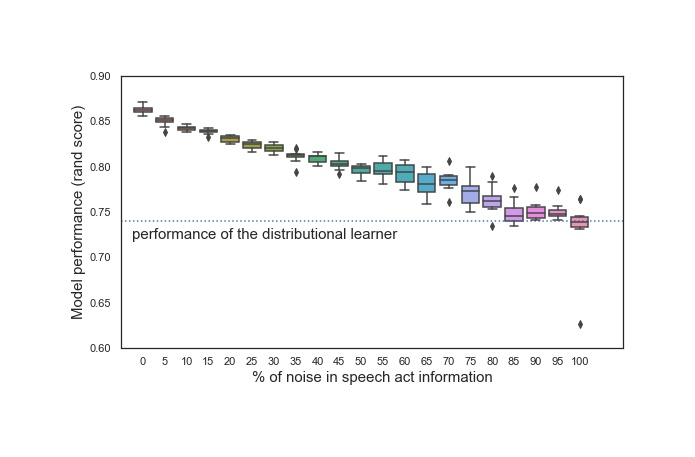
\includegraphics[width=1\textwidth]{figures/noisy-rand-compare.jpg}
    \caption{Compare the performance of pragmatic distributional learners taking different levels of noisy speech act information; dotted marks the rand score of the distributional learner}
    \label{fig:noisy-rand-compare}
\end{figure}

Looking at the learner at maximum noise level, we can see that the model fails to identify a cluster for declaratives (Figutre~\ref{fig:noisy100-heatmap}. Similar to the distributional learner, the cluster for imperatives also have declaratives (\ref{fig:noisy100-heatrev}). 



\begin{figure}[H]
    \centering
    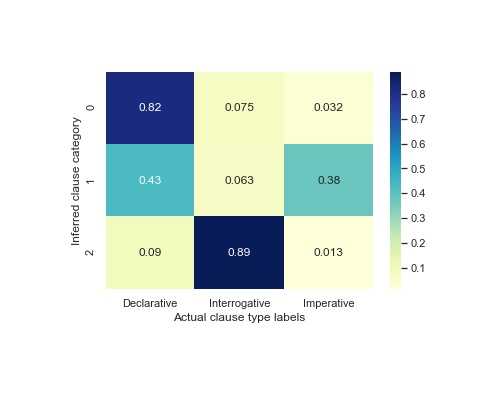
\includegraphics[width=0.7\textwidth]{figures/noisy100-heatmap.jpg}
    \caption{The proportion of \diis{} in each of the three clusters (100\% noise in speech act information) }
    \label{fig:noisy100-heatmap}
\end{figure}

\begin{figure}[H]
    \centering
    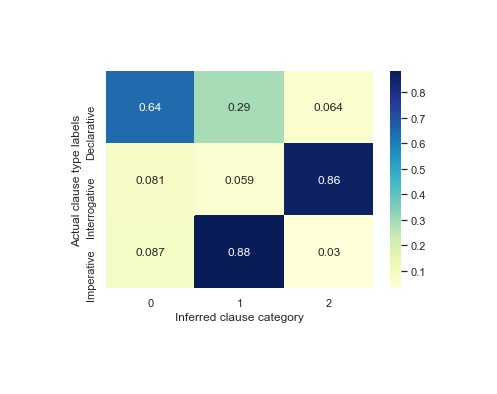
\includegraphics[width=0.7\textwidth]{figures/noisy100-heatrev.jpg}
    \caption{The proportion of actual \diis{} clustered in one category}
    \label{fig:noisy100-heatrev}
\end{figure}

Looking at the distribution of syntactic features, we can see that the model has the same problem as the distributional learner. Cluster $0$, which should be the imperative cluster, still have sentences that have subjects. 

\begin{figure}[H]
    \centering
    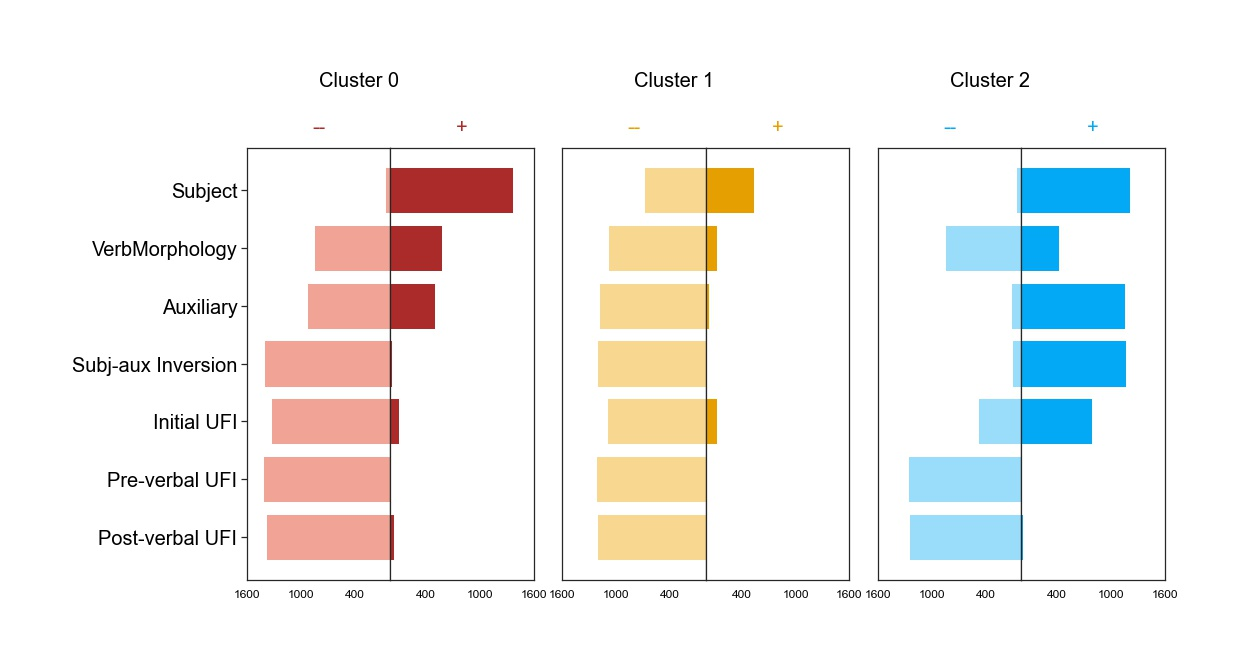
\includegraphics[width=1\textwidth]{figures/noisy100-syncluster.jpg}
    \caption{The number of sentences with/without certain formal features in each cluster (Cluster 0 $\sim$ Interrogatives, Cluster 1 $\sim$ Imperatives, Cluster 2 $\sim$ Declaratives), darker colors represent the number of sentences with the feature.}
    \label{fig:noisy100-syncluster}
\end{figure}




\subsection{Interim Discussion}
\label{sec:engcl:model:disc}
In summary, the speech act information is very tolerant of noises. The pragmatic distribution learner consistently outperforms the distributional learner, and only drops when the noise in speech act reaches 85\%. 

These results suggest that pragmatic information is crucial to the learner, not just to solve the labeling problem, but also to help with clustering. 

\section{Discussion}
\label{sec:engcl:discussion}

In this chapter, we looked at how learners might learn to categorize sentences. We first examined the patterns in parents' input, and see that parents use clause types systematically, and that the three clause types are predominantly mapped to their canonical functions (declaratives to assertions, interrogatives to questions, imperatives to requests/commands). The three clause types are also used systematically, with their formal features consistently present in the input sentences. 

We then address the question of how infants might succeed at the clustering task. Specifically, do they need pragmatic information to solve the clustering problem? Given the fact that clause types are formal categories, it is at first glance reasonable to assume that infants are able to identify the main clause types with formal features only. We build two learners, the distributional learner and the pragmatic distributional learners to probe this question. The distributional learner learns clause typing from formal features only, but the pragmatic distributional learner also has access to the speech act information. We find that the pragmatic distributional learner outperforms the distributional learner, suggesting that pragmatic information is necessary, even for clustering. We then manipulated the level of noise in speech act, to see how tolerant this information source can be. Turns out, even if the pragmatic distributional learner is given speech act information with 85\% of noise, they still outperforms the distributional learner. 

From these results, we conclude that pragmatics is essential for learning clause typing. Infants learn how to cluster sentences into clause types by observing the formal features of the sentences, together with speech act information.



The question remains is that, how does the pragmatic distributional learner identify speech act information? While it is indisputable that information from clause type should be necessary, are there any non-clause type information about speech act in their everyday interaction with parents? In Chapter~\ref{chap:eng-sp}, we will turn to the learning of speech acts from non-clause type information.


Another question is, what about other languages? As we have discussed in Chapter~\ref{chap:litreview}, languages differ in the formal features of each clause type, and learners need to discover the correlation from input. The distributional learner for English still have some success with clustering, identifying interrogative clauses. However, maybe the formal features are not as informative in other languages. In the next chapter, we will turn to Mandarin learners, and test the two learners with Mandarin input data. 

